\begin{frame}
\frametitle{Intersection automata construction}

 \tiny{\textcolor{blue}{Let us consider the two B\"{u}chi automatons P and Q, %as shown in Fig \ref{fig1} 
and defined by the conventional five tuple:}}

\tiny{\textcolor{blue}{$P = \{(p_0,p_1),(a,b),p_0, Q \times \sum \rightarrow Q,p_1\}$}}

\tiny{\textcolor{blue}{$Q = \{(q_0,q_1),(a,b),q_0, Q \times \sum \rightarrow Q,q_1\}$}}



\begin{figure}
\begin{center}
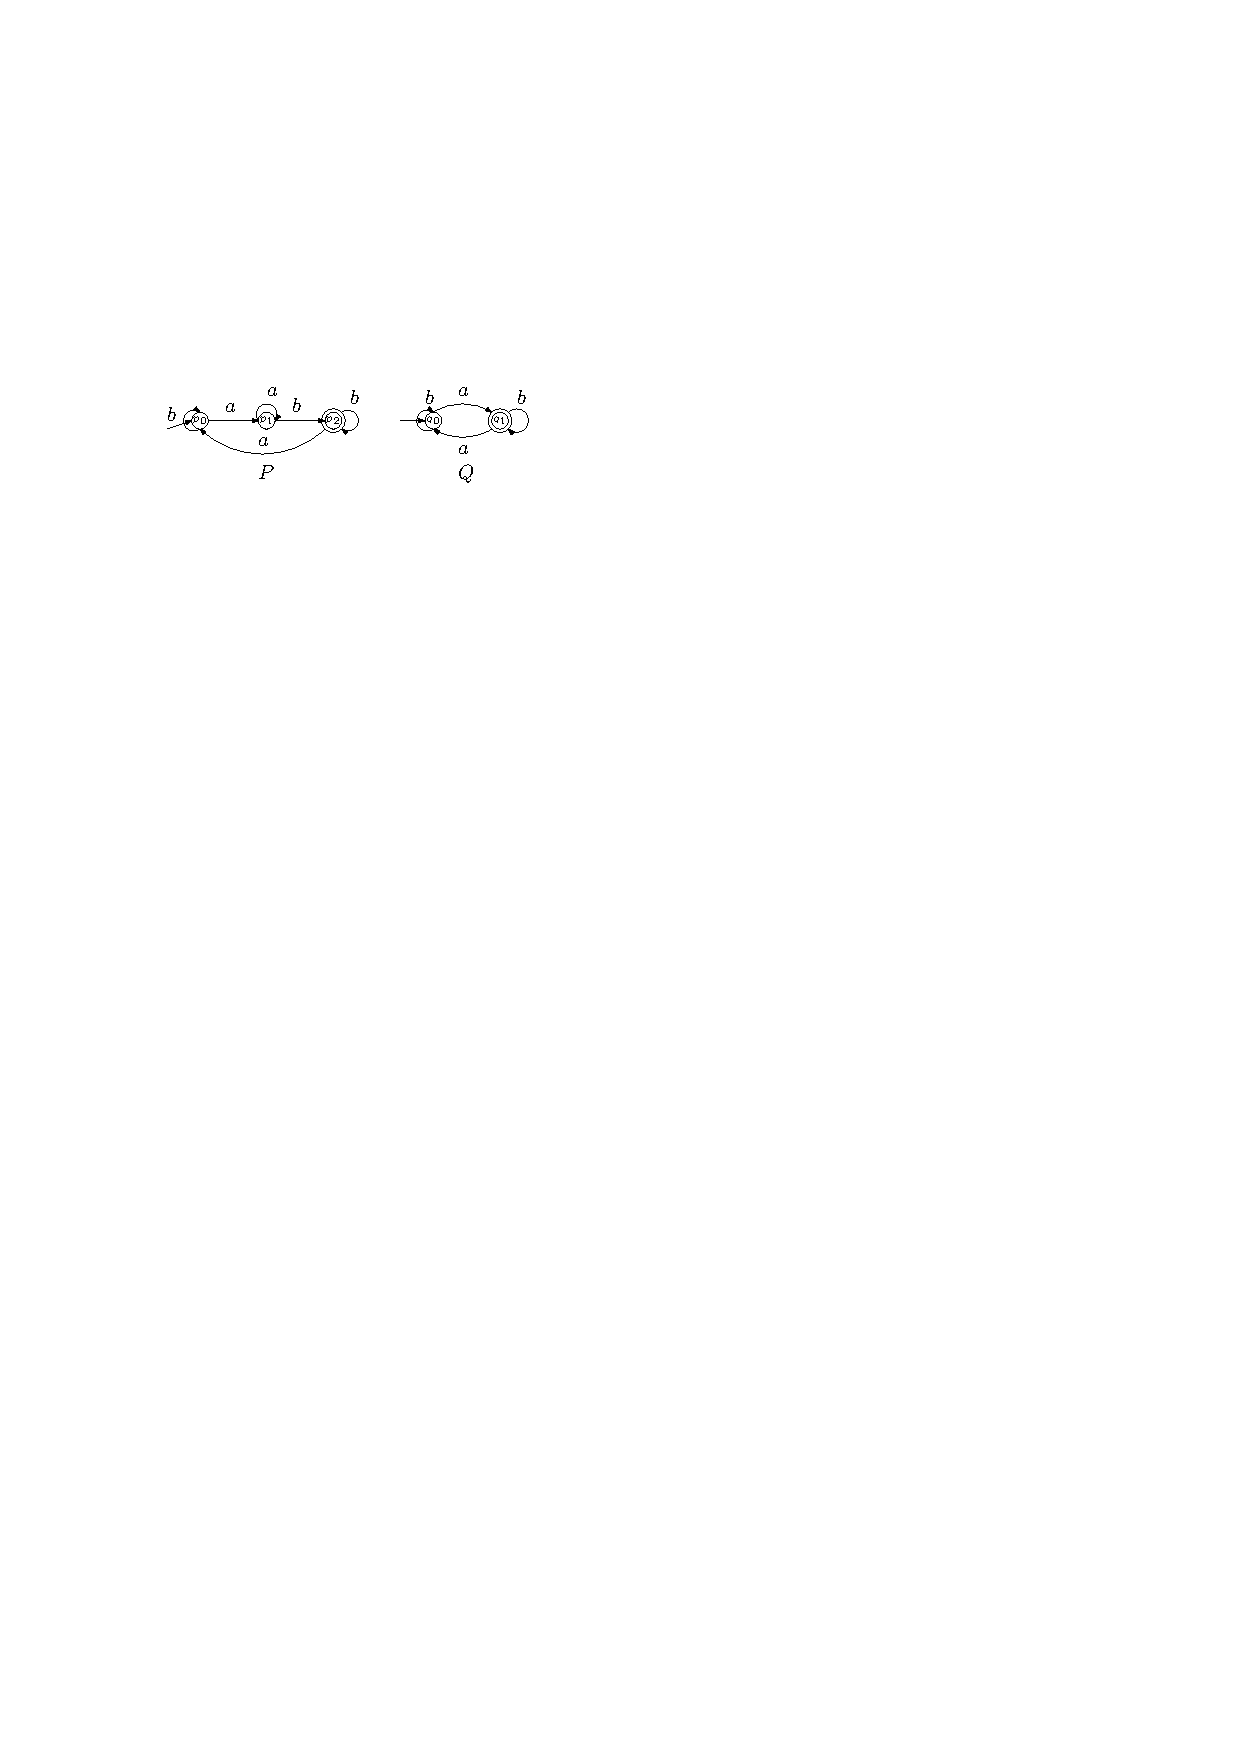
\includegraphics[width=45mm]{example_1.pdf}
\end{center}
%\vspace{-0.1in}
\caption{{\em \tiny{\textcolor{blue}{Individual automatons}}}} \label{fig1}
\end{figure}


\tiny{\textcolor{blue}{Considering  the reachable states, starting from the start 
state, the intersection automata of the given input automatons is given below.}}


 \begin{figure}
\begin{center}
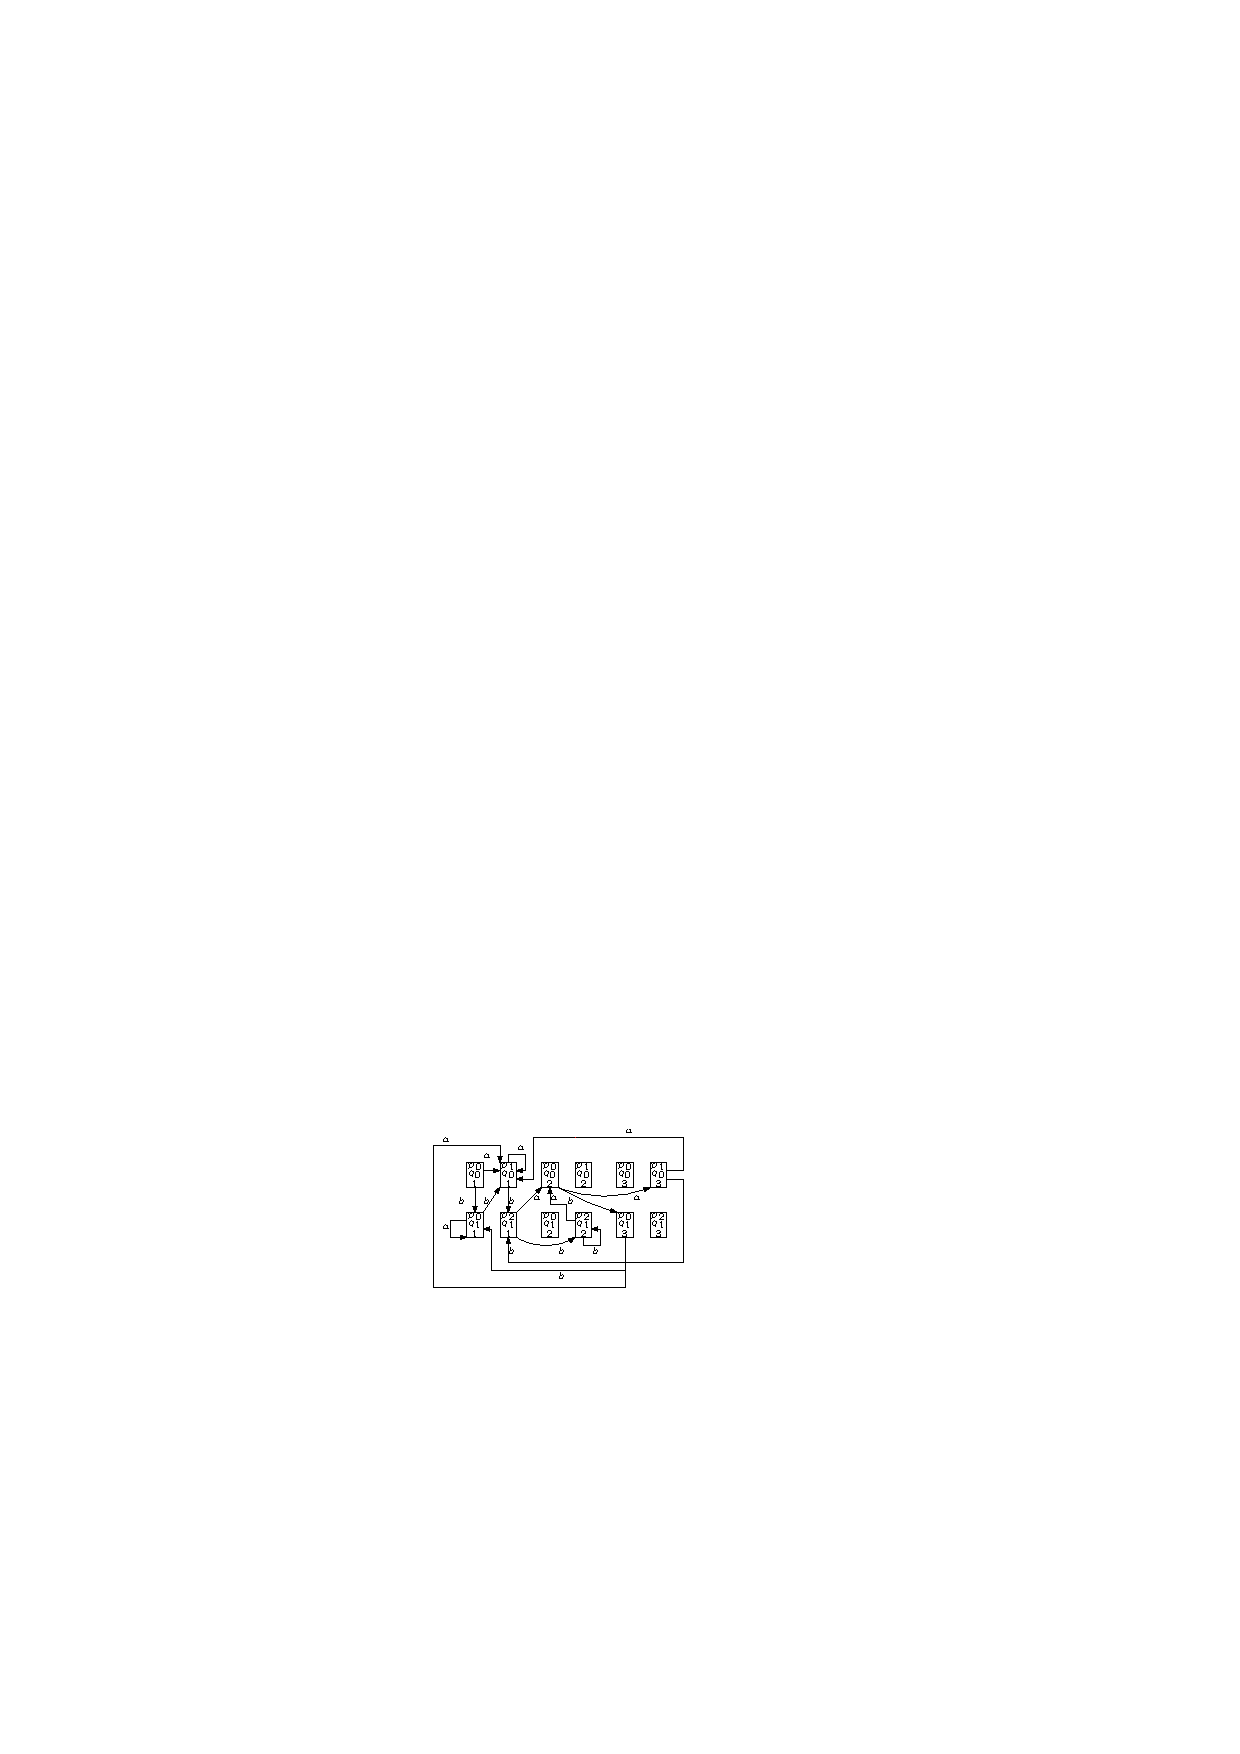
\includegraphics[width=40mm]{state_copy_transition.pdf}
\end{center}
%\vspace{-0.1in}
\caption{{\em\tiny{\textcolor{blue}{ Intersection of the input automata}}}}
\label{transition}
\end{figure}
% 
%  \begin{figure}
% \begin{center}
% %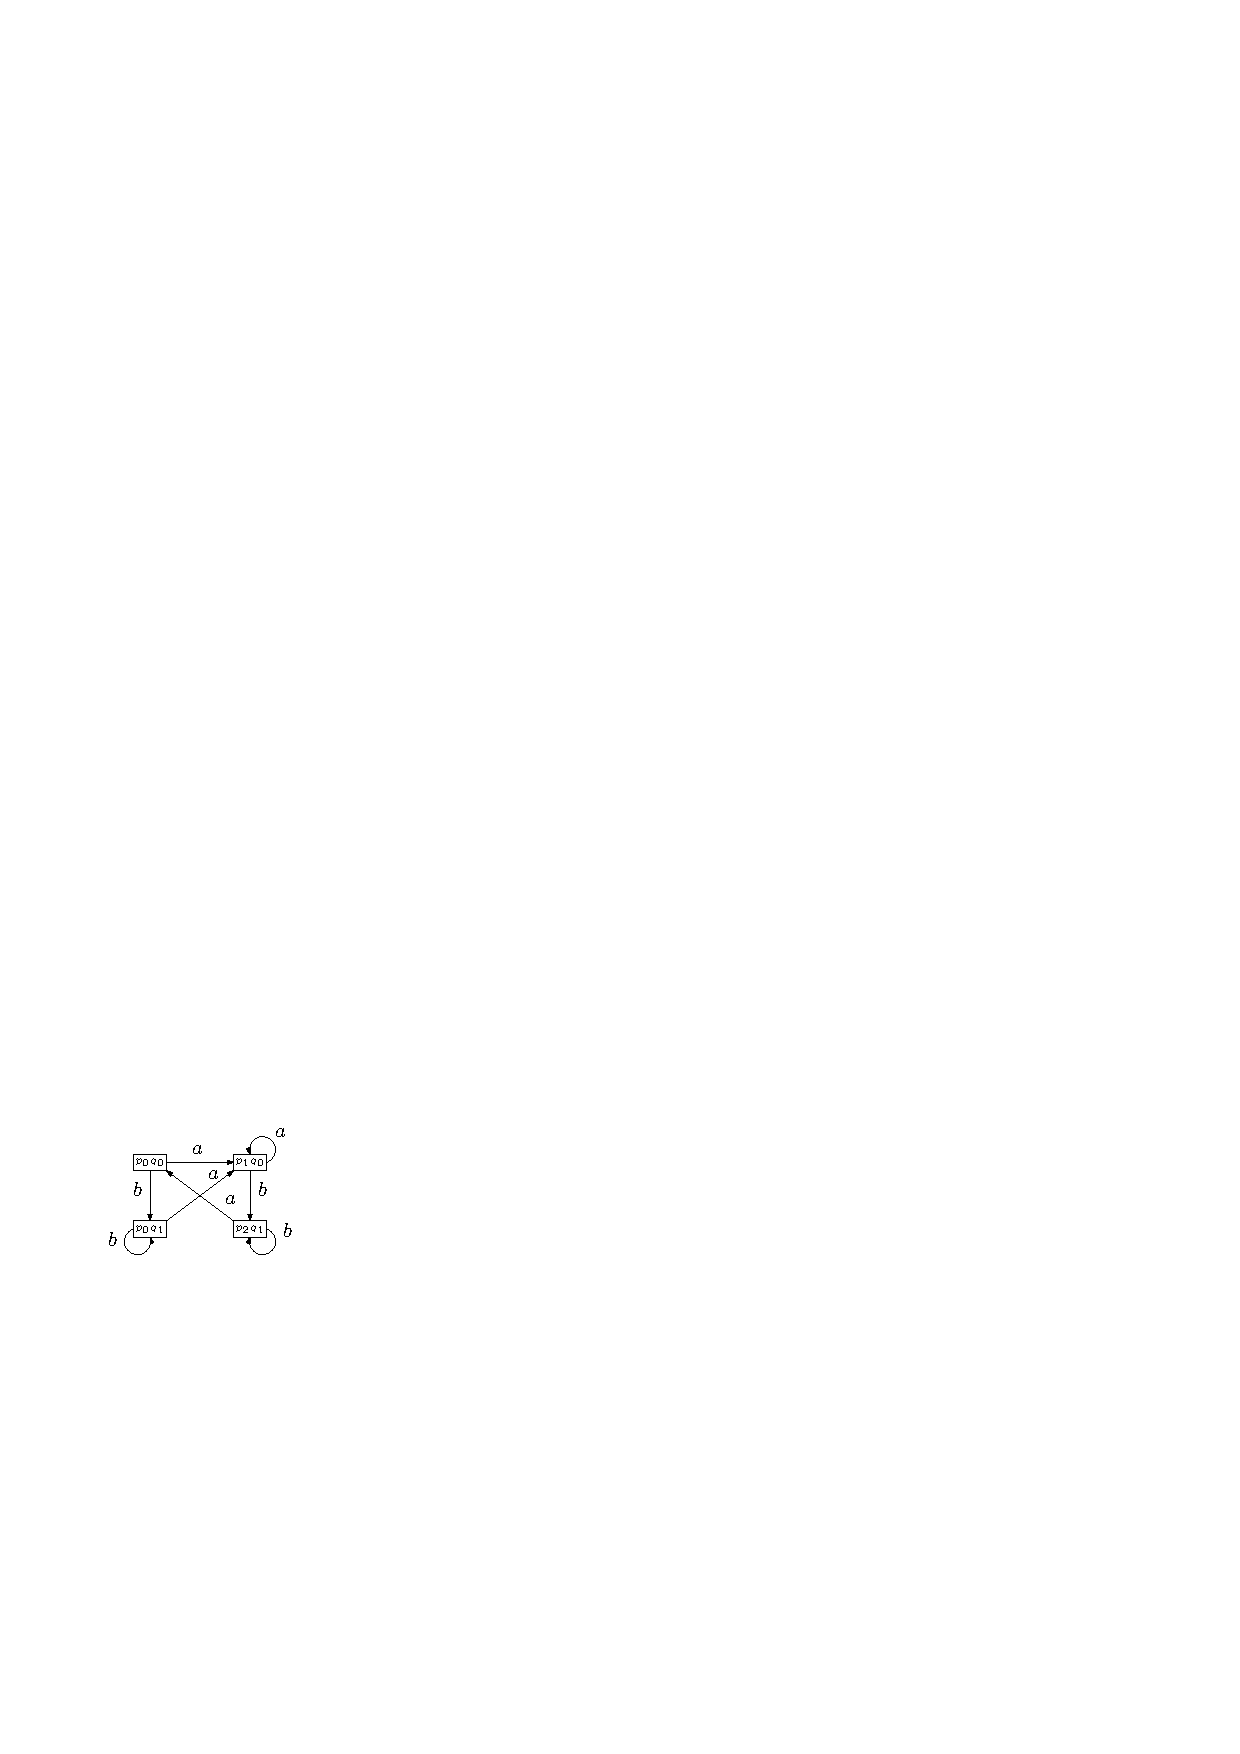
\includegraphics[width=50mm]{product.pdf}
% \end{center}
% %\vspace{-0.1in}
% %\caption{{\em Intersection of the input automata}}
% \label{product}
% \end{figure}
 

% \tiny{\textcolor{blue}{Intersection of B\"{u}chi automatons require a special handling to model
% the infinitary acceptance condition on top of the classical product construction 
% of finite automatons. We can see in Fig~\ref{product} that the states do
% not contain the tuple $<p_2,q_0>$, the set of final states
%  from both the automata. In  the following steps, we modify the product construction to include accepting states from
%  both the automata. The resulting intersection automata ensures that accepting states of
%  both the automatons are visited  infinitely often. From the set of states of each
%  individual automaton, where each state is reachable from the 
%  start state, we make three copies of the product automata. In general, for $n$
%  such automatons, $n$+$1$ copies are made.
%  Each copy has a flag with the states, as shown in Fig\ref{fig:copy}. The flags 
%  associated with  the states are waiting to see the acceptance of the automaton.
% In Fig \ref{fig:copy}, flag $1$ is waiting to see the acceptance state of P, flag $2$ is waiting to see
% the acceptance state of Q, and states with flag $3$ signify that the track has traversed all the accepting states
% of both the automatons. Starting from the first copy, the transitions are made according to the product automaton.
%  A transition goes to the next flag if it gets the final state of one automaton. In general, for an automaton state 
%  associated with this flag in the product, if the acceptance condition of an automaton is obtained, the transition
%  goes to the next copy, otherwise it remains within the transitions on its own states, as shown in  Fig\ref{transition}.
%  When it reaches the last copy, it has traversed the accepting state of
%  each individual automaton. The red cycle in Fig~\ref{transition} shows one such cycle. After reaching the last
%  state, it goes to the first state. In the resulting automaton, a cycle is accepted, when it passes through the last copy
%  of the product automaton, that signifies the run of the cycle traverses the accepting states of each automaton
%  infinitely often. The remaining cycles, which do not pass through the last copy, are not accepted. We thus augment 
%  the classical product construction for finite automatons to model our infinitary acceptance requirement.}}
 
% \begin{figure}
% \begin{center}
% %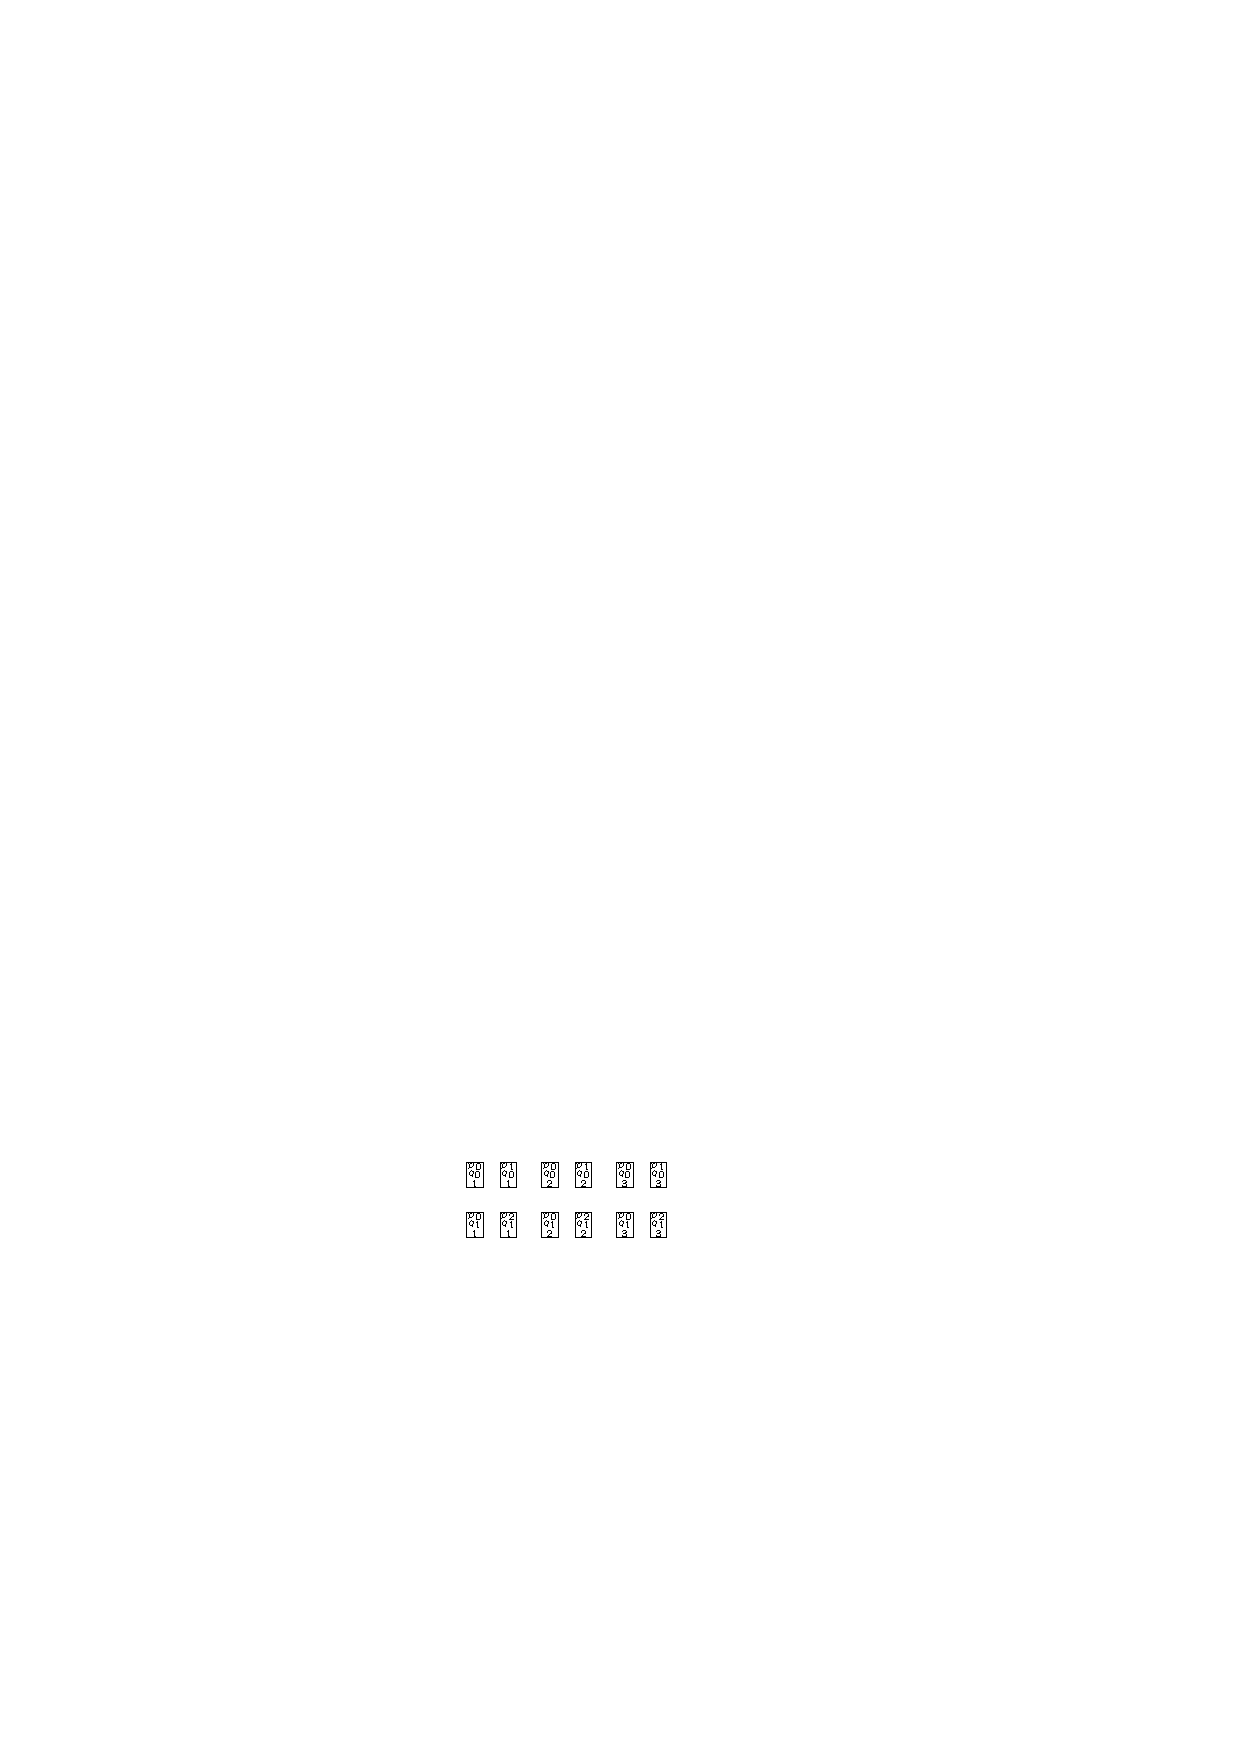
\includegraphics[width=50mm]{state_copy.pdf}
% \end{center}
% %\vspace{-0.1in}
% %\caption{{\em Product automata construction with flags}}
% \label{fig:copy}
% \end{figure}

 


\begin{figure}
\begin{center}
%\includegraphics[width=50mm, height=75mm]{algorithn.pdf}
\end{center}
%\vspace{-0.1in}
%\caption{{\em Flow chart of our idea}}
\label{fig:Algorithm}
\end{figure}

\end{frame}
